\documentclass{article}

\usepackage{amsmath,amsfonts,amssymb}
\usepackage{graphicx}
\usepackage{xspace}
\usepackage{titlesec}
\usepackage{algorithm,algorithmic}
\usepackage{subfig}
\usepackage{latexsym}

% Latin abbreviations
\newcommand\etal{\textit{et al.}\xspace}
\newcommand\ie{\textit{i.e.}\xspace}
\newcommand\eg{\textit{e.g.}\xspace}
\newcommand\cf{\textit{c.f.}\xspace}
\newcommand\etc{\textit{etc.}\xspace}

% References
\newcommand\figref[1]{Figure \ref{fig:#1}}
\newcommand\Figref[1]{Figure \ref{fig:#1}}
\newcommand\secref[1]{Section \ref{sec:#1}}
\newcommand\Secref[1]{Section \ref{sec:#1}}
\newcommand\sectref[1]{Section \ref{sec:#1}}
\newcommand\Sectref[1]{Section \ref{sec:#1}}
\newcommand\chapref[1]{Chapter \ref{chap:#1}}
\newcommand\Chapref[1]{Chapter \ref{chap:#1}}
\newcommand\tableref[1]{Table \ref{table:#1}}
\newcommand\Tableref[1]{Table \ref{table:#1}}
\newcommand\algref[1]{Algorithm \ref{alg:#1}}
\newcommand\Algref[1]{Algorithm \ref{alg:#1}}
\newcommand\eqnref[1]{\eqref{eq:#1}}

% Counters
\renewcommand\th[0]{\textsuperscript{th}\xspace}
\newcommand\st[0]{\textsuperscript{st\xspace}}
\newcommand\nd[0]{\textsuperscript{nd\xspace}}
\newcommand\rd[0]{\textsuperscript{rd\xspace}}

% Generic math
\newcommand\degrees{^\circ}
\newcommand\vect[1]{\boldsymbol{#1}}
\newcommand\grad{\nabla}
\newcommand\xor{\oplus}
\newcommand\union\cup
\newcommand\abs[1]{\lvert#1\rvert}
\newcommand\norm[1]{\lVert#1\rVert}
\DeclareMathOperator*\argmax{argmax}
\DeclareMathOperator*\argmin{argmin}
\newcommand\cross\times
\newcommand\concat{\ensuremath{+\!\!\!\!+\,}}
\newcommand\sign{\operatorname{Sign}}

% Analysis
\newcommand\intd{\mathrm{d}}   % for the 'dx' in integrals
\newcommand\NormalDistr{\mathcal{N}}
\newcommand\Expected{\mathbb{E}}
\newcommand\Deriv[2]{\frac{\partial #1}{\partial #2}}
\newcommand\EvalAt[1]{\biggl|_{#1}}

% Fields
\newcommand\field[1]{\mathbb{#1}}
\newcommand\Reals{\field{R}}
\newcommand\Rtwo{\Reals^2}
\newcommand\Rthree{\Reals^3}
\newcommand\Rfour{\Reals^4}
\newcommand\Ints{\field{Z}}

% Theorems
%\newtheorem{theorem}{Theorem}
%\newtheorem{lemma}{Lemma}
%\newtheorem{corollary}{Corollary}
%\newtheorem{definition}{Definition}


\newcommand\Hcf{H_{c \rightarrow f}}
\newcommand\Hcfhat{\hat{H}_{c \rightarrow f}}

\newcommand\vvpt{\vect{v_v}}
\newcommand\lvpt{\vect{v_l}}
\newcommand\rvpt{\vect{v_r}}

\newcommand{\abs}[1]{\lvert#1\rvert}
\newcommand{\norm}[1]{\lVert#1\rVert}


\newcommand\Payoff{\Pi}
\newcommand\ColPayoff{\pi}
\newcommand\Model{M}
\newcommand\ManhattanClass{\mathcal{M}}
\newcommand\Feature{\vect{\psi}}
\newcommand\Features{\Psi}
\newcommand\Pixel{\vect{p}}
\newcommand\Pixels{\vect{P}}
\newcommand\Orient{a}
\newcommand\Depth{d}
\newcommand\Depths{D}
\newcommand\Ind{t}

\newcommand\Penalties{\vect{\lambda}}
\newcommand\PenaltyOccl{\lambda_\textsf{occl}}
\newcommand\PenaltyConc{\lambda_\textsf{conc}}
\newcommand\PenaltyConv{\lambda_\textsf{conv}}

\newcommand\tIN{\tau_{\textsf{IN}}}
\newcommand\tOUT{\tau_{\textsf{OUT}}}
\newcommand\tON{\tau_{\textsf{ON}}}


\newcommand\fIN{f_{\textsf{in}}}
\newcommand\fOUT{f_{\textsf{out}}}
\newcommand\fUP{f_{\textsf{up}}}
\newcommand\fDOWN{f_{\textsf{down}}}

\input GotIn.fd
\newcommand*\initfamily{\usefont{U}{GotIn}{xl}{n}}

\begin{document}

\section{Abstract}

\section{Introduction}

\initfamily
\fontsize{50}{60}
\selectfont
O\fontsize{10}{12}\normalfont ver the past decade, computer vision researchers working with
monocular images have pursued substantially different research
directions to those working with multiple views. The focus for
monocular images has increasingly been to infer high--level facts
about the world, such as the locations of and interactions between
objects, to semantic scene categories and the spatial layout of the
environment. In constrast, much of the work concerning multiple views
has focussed on reconstructing camera poses and scene structure using
techniques such as structure--from--motion, stereo, and multiple--view
stereo, with performance metrics typically concerned with geometric
accuracy of the reconstructions.

In this paper we focus on utilizing multiple view geometry for image
understanding purposes. We assume a moving camera with a
structure--from--motion system estimating its trajectory through
space, and show how to infer semantically meaningful models of the
environment. We focus on the \textit{indoor Manhattan
  representation}\cite{Lee09}, in which the world is modelled
in terms of floor, wall, and ceiling surfaces. This representation
captures many semantically meaningful aspects of the environment,
including
\begin{enumerate}
  \item{\textbf{Scale}: the distance from floor to ceiling suggests
    a scale for distances in the environment}
  \item{\textbf{Boundaries}: walls constrain movement in the
    environment and suggest locations for doors, windows, and other
    objects.}
  \item{\textbf{Gravity}: the orientation of the ground plane implies
    the direction in which gravity operates, which constrains the
    arrangement of objects resting upon one another.}
  \item{\textbf{Shape}: the organisation of walls in an environment
    suggests its functional category (kitchen/office/etc).}
\end{enumerate}

Indoor manhattan models are useful because they capture these
properties explicitly as primitives of the model, whereas to extract
such properties from a dense polygonal mesh reconstruction would
require additional non--trivial inference following the reconstruction
stage. Our approach can be seen as inferring semantic properties of
the scene directly from multiple--view data, without an intermediate
dense reconstruction step. This makes sense if, as is the case in our
context, these proprties constitute the ultimate goal of the
system. Of course, if a photo--realistic reconstruction is itself the
end goal then our approach is not suitable.

We build on the dynamic programming approach to inferring indoor
manhattan models of Flint \etal \cite{FlintECCV10}. Our work extends
their approach to allow joint inference across multiple views as well
as to incorporate range data alongside photometric cues. This involves
a significant generalization of their approach since neither of these
new modalities are representable using their pixel--wise cost
function. We therefore generalize their approach to a payoff--based
formulation permitting more general costs. We also show that in this
new formulation one of the state variables involved in their
optimisation is unecessary; its removal corresponds to eliminating an
entire dimension from the search and results in an order of magnitude
efficiency improvement.

XXX Probabilistic cost function

XXX Combine monocular, multi-view, and range features

When comparing our approach to previous work we propose that in
addition to measuring geometric accuracy, the \textit{size} of
alternative representations should also be compared, since models that
capture key properties of the environment using fewer representational
bits must have done a better job of filtering salient information
from sensor data. This is in line with the relationship between the
ability of an algorithm to compress data and its ability to make
predictions (cite Hutter).

The remainder of this paper is organised as follows. XXX

\section{Background}

The Manhattan world assumption has seen increasing attention in the
computer vision literature over past years
\cite{Coughlan99,Zhang02,Lee09,Furukawa09,FlintECCV10}. It was
introduced by Coughlan and Yuille\cite{Coughlan99} for estimating
camera orientations. Furukawa \etal \cite{Furukawa09} proposed a
``Manhattan--world stereo'' algorithm that incorporates Manhattan
orientations into an energy function, which they solve using graph
cuts. 

Brostow et al

Talk more about multi view reconstructions

BUILDING RECONSTRUCTION USING MANHATTAN WORLD GRAMMARS

The ECCV(?) paper on using manhattan + non-manhattan surfaces for
reconstruction.

While their approach is concerned with dense photo--realistic
reconstructions, ours is intended to capture semantic properties of
the scene using a representation that is as concise as possible.

Lee \etal \cite{Lee09} first proposed indoor Manhattan models (a
sub--class of general Manhattan models) for monocular
reconstructions. They used a branch--and--bound algorithm together
with a line--sweep heuristic for approximate inference. Flint \etal
\cite{Flint10ECCV} inferred similar models using a dynamic programming
algorithm. In earlier work \cite{Flint10CVPR} they demonstrated
Manhattan reconstructions integrated with a SLAM system, but this work
inferred models from single frames and then extrapolated these forward
in time. In contrast, the present work allows both photoconsistency
and depth information to be included directly in the cost function,
allowing far more robust inference.

XXX We also use features and learning rather than a line sweep heuristic...

Felzenszwalb and Veksler \cite{Felzenszwalb10} posed the
reconstruction problem in terms of an energy minimisation, which they
showed could be solved using dynamic programming. Barinova \etal
\cite{Barinova08} proposed to model outdoor scenes using a conditional
random field over vertical plane boundaries. However, neither of these
approaches capture the geometry of indoor Manhattan scenes in the
strong sense, and neither of them optimize over cost functions that
can incorporate multiple views or depth data.

\section{Model}

\begin{figure}[tb]%
  \centering
  \label{fig:ideal-models}
  \begin{tabular}{ccc}
    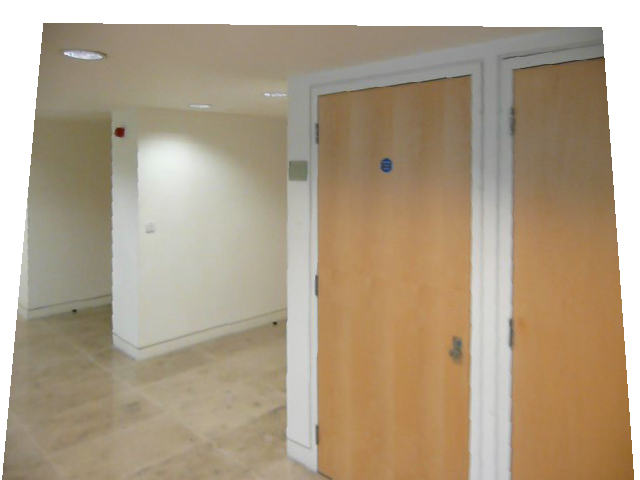
\includegraphics[width=0.2\textwidth]{figures/true_models/lab_ground1_010_rect.png} &
    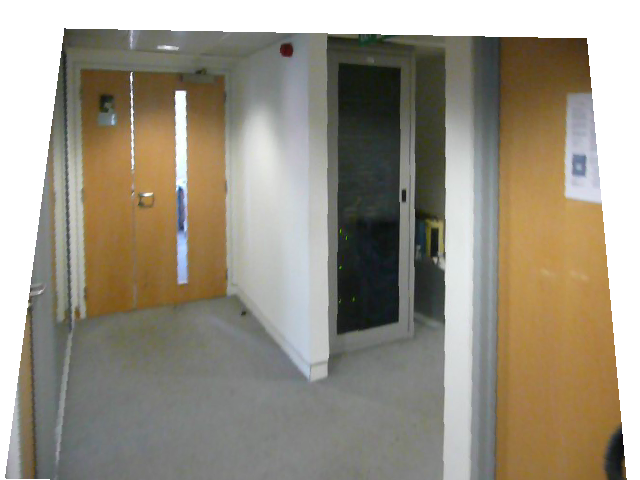
\includegraphics[width=0.2\textwidth]{figures/true_models/lab_kitchen_030_rect.png} &
    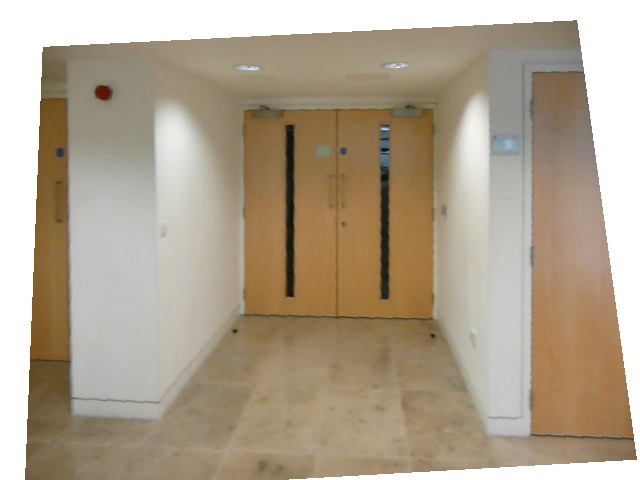
\includegraphics[width=0.2\textwidth]{figures/true_models/lab_ground1_030_rect.png} \\
    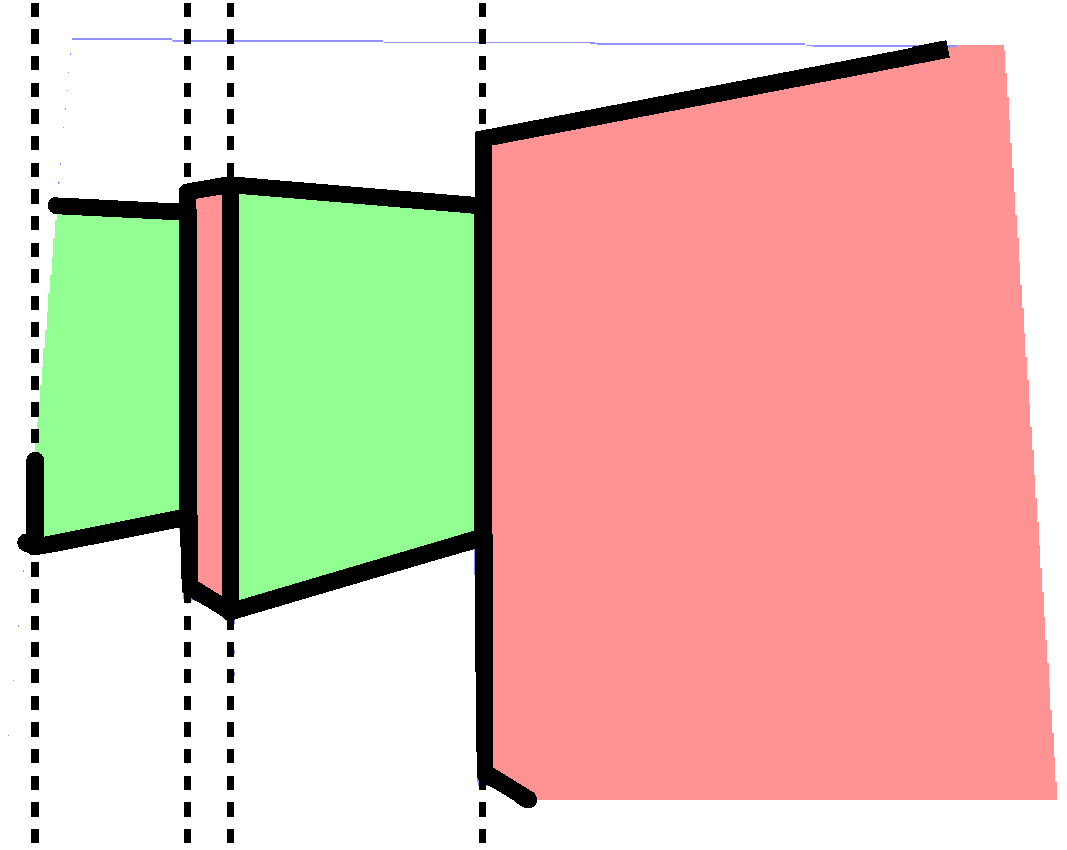
\includegraphics[width=0.2\textwidth]{figures/true_models/lab_ground1_010} &
    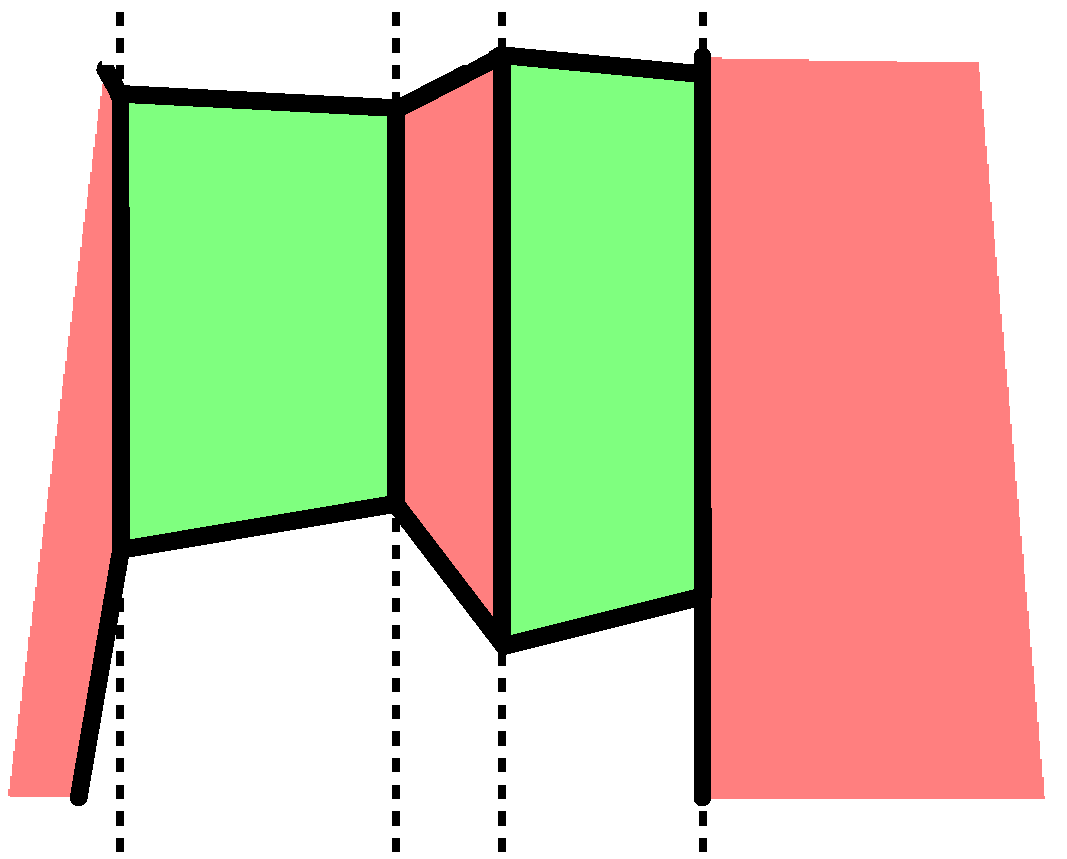
\includegraphics[width=0.2\textwidth]{figures/true_models/lab_kitchen_030} &
    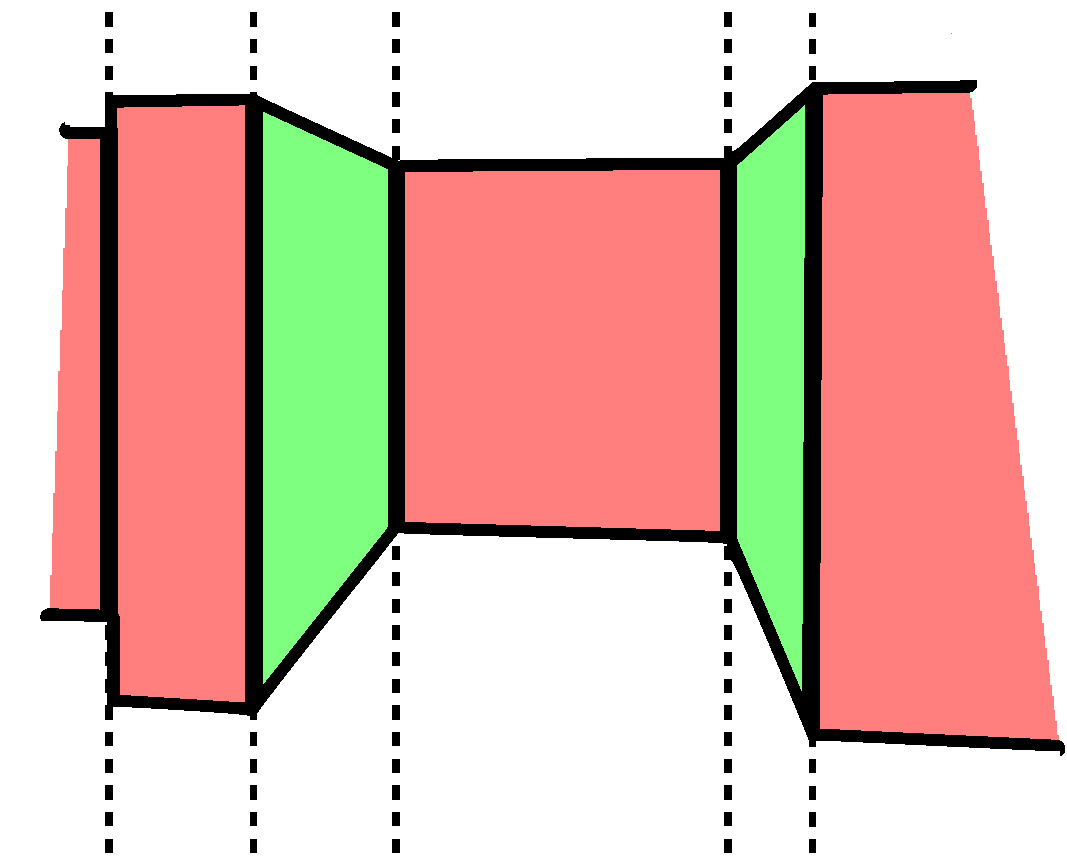
\includegraphics[width=0.2\textwidth]{figures/true_models/lab_ground1_030}
  \end{tabular}
  \hspace{0.2cm}
  \caption{Three input images and the indoor Manhattan models we
    seek. Notice how each image column intersects exactly one
    wall.}
\end{figure}

In this section we describe the class of indoor Manhattan models and
pose inference within this class as maximization of a payoff function
that decomposes over image columns. In subsequent sections we will
show that reasonable generative models for photometric,
multiple--view, and depth features give rise to MAP inference formulae
that decompose in precisely this way, so that, given appropriate
mapping of sensor inputs to payoffs, maximization of the payoff
function is equivalent to MAP inference in a graphical model. This
will allow us in \sectref{inference} to provide a concise dynamic
programming solution in the setting of payoff matrices.

An indoor Manhattan model consists of a floor plane, a parallel
ceiling plane, and a set of vertical walls extending between
them. Each wall extends all the way from the floor to ceiling, and
pairs of walls meet at vertical edges. Walls are restricted to two
orthogonal orientations, and the camera is assumed to be located
between the floor and ceiling planes.

We always consider indoor Manhattan models as seen from a particular
camera. In can be shown that, due to the assumption of walls extending
all the way from floor to ceiling, indoor Manhattan models always
project as a sequence of walls that only ever meet (in the image) their
left and right neighbours (in the sequence).

We assume that vanishing points for each of the three Manhattan
directions are given. There are several well--known techniques for
extracting vanishing points from images\cite{Shufelt99}; for the
monocular case we use the EM approach of \cite{Zhang02}, and in the
multiple view setting we use the joint estimation approach of
\cite{FlintCVPR10}.

It will simplify the remainder of this paper if we assume that
vertical lines in the world appear vertical in images. Given the
location of the vertical vanishing point $\vvpt$ we rectify images
according to the homography
\begin{equation}
  H = 
  \begin{pmatrix}
    \vvpt \times \vect{e_3} \\
    \vvpt \\
    \vvpt \times \vect{e_3} \times \vvpt
  \end{pmatrix}
  ~,~~~~~~~~ \vect{e_3}=[0,0,1]^T ~.
\end{equation}
This will introduce warping artifacts for cameras with a
near--vertical principal ray; however, this rectification step is not
strictly necessary and we could instead perform geometric calculations
in the original image coordinates, though doing so would signficantly
complicate the exposition of this paper.

Following rectification in can be shown that each image column
contains exactly one wall segment; for example, see
\figref{ideal-models}. Let the position of the floor--wall boundary in
image column $x$ be $y_f(x)$, and the position of the corresponding
ceiling--wall boundary be $y_c(x)$. We define the payoff
$\Payoff(\Model)$ for the model $\Model$ as
\begin{equation}
  \label{eq:abstract-payoffs}
  \Payoff(\Model) = \sum_x \Bigl(\ColPayoff(x,y_f) +
  \ColPayoff(x,y_c)\Bigr) ~.
\end{equation}
where $a$ is a payoff matrix assigning to each pixel a payoff for
models that label that pixel as a floor-wall or ceiling--wall
intersection. Note that $a(x,y)$ is \textit{not} restricted to
dependence on pixel $(x,y)$, or even to a local region about $(x,y)$,
and indeed the payoff functions described in the next section
incorporate image evidence from image regions far from $(x,y)$.

Where to put this?? Since the 3D points corresponding to $y_c$ and
$y_f$ are vertically above/beneath one another, and because the floor
and ceiling planes are parallel to one another, $y_c$ and $y_f$ are
related to one another via a planar homology\cite{Criminisi01} $G$,
\begin{equation}
  \begin{pmatrix} x \\ y_c \\ 1 \end{pmatrix}
  \hspace{0.3cm} \sim \hspace{0.3cm}
  G \begin{pmatrix} x \\ y_f \\ 1 \end{pmatrix}
  ~.
\end{equation}

TODO: how to incorporate penalties for additional walls etc.

\subsection{Monocular features}

\begin{figure}[tb]
  \centering
  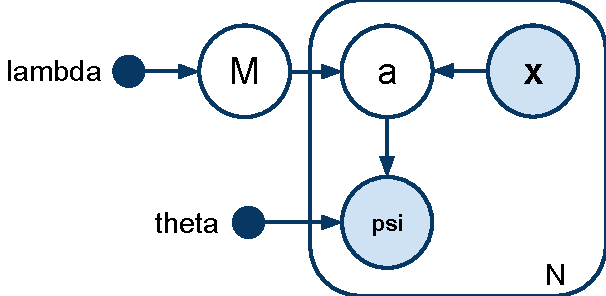
\includegraphics[width=0.5\textwidth]{figures/monocular-gm}
  \caption{The graphical model relating building structures $M$ to
    monocular image features $\Feature$. $\Pixel=(x,y)$ is an observed
    pixel location and $a$ is indicates the orientation of the model
    $M$ at that pixel.}
  \label{fig:monocular-gm}
\end{figure}

To infer indoor Manhattan models from monocular images we assume the
graphical model shown in \figref{monocular-gm}. Pixel features
$\Feature$ are dependent on the orientation $\Orient\in\{1,2,3\}$ at
that pixel, where the possible values for $\Orient$ correspond to the
three manhattan orientations. We assume a linear model for pixel
features,
\begin{equation}
\label{eq:feature-likelihood}
  P(\Feature ~|~ \Orient) =
  \frac{{\vect{\theta}_\Orient}^T\Feature}
       {\sum_j{\vect{\theta}_\Orient}^T\Feature_j} ~.
\end{equation}

A model $\Model$ generates pixel orientations $\Orient$
deterministically. We include this variable for notational
convenience only, thus
\begin{equation}
  \label{eq:orient-model}
  P(\Orient ~|~ \Model,\Pixel) = 
    \begin{cases}
      1, & \mbox{if } \Orient = a^*(\Model,\Pixel) \\
      0, & \mbox{otherwise}\\
    \end{cases}
    ~,
\end{equation}
where $a^*(\Model,\Pixel)$ denotes the orientation predicted by model
$\Model$ at pixel $\Pixel$, which we compute by filling polygons in
the image. Finally, for a model with $n_1$ concave corners, $n_2$
convex corners, and $n_3$ occluding corners, we assume the complexity
prior
\begin{eqnarray}
  \label{eq:model-prior}
  P(\Model ~|~ \Penalties) &=& \frac{1}{Z} 
    \PenaltyConc^{n_1} \PenaltyConv^{n_2} \PenaltyOccl^{n_3} \\
  Z &=& \sum_{n_c,n_n,n_o} P(\Model ~|~ \Penalties) \\
    &=& \frac{1}{(1-\PenaltyConc)(1-\PenaltyConv)(1-\PenaltyOccl)}
\end{eqnarray}
This corresponds to a fixed probability for ``events'' corresponding
to each type of corner. XXX need to introduce the three types of
corners earlier.

We now derive MAP inference for indoor manhattan models. The posterior
on building structures given observed image features is
\begin{eqnarray}
  P(\Model ~|~ \Features,\Pixels) &=&
  \eta P(\Model) P(\Features,\Pixels ~|~ \Model)
  \\
  &=& \eta P(\Model) \prod_i P(\Feature_i,\Pixel_i ~|~ \Model)
  \\
  &=& \eta \sum_A P(\Model) \prod_i
    P(\Feature_i,\Pixel_i, \Orient_i  ~|~ \Model)
  \\
  &=& \eta \sum_A P(\Model) \prod_i P(\Feature_i ~|~ \Orient_i)
    P(\Orient_i ~|~ \Pixel_i,\Model) ~.
\end{eqnarray}
But according to \eqnref{orient-model}, the only non--zero term in the
summation over $A=\{a_i\}_{i=0}^N$ is the one for which $a_i =
  a_i^*(\Model,\Pixel_i)$. Hence,
\begin{eqnarray}
  \label{eq:mono-post}
  P(\Model ~|~ \Features,\Pixels) &=&
  \eta P(\Model) \prod_i P(\Feature_i ~|~ \Orient_i^*) \\
  \label{eq:mono-logpost}
  \log P(\Model ~|~ \Features,\Pixels) &=&
  c + n_1 \log \PenaltyConc + n_2 \log \PenaltyConv + n_o \log \PenaltyOccl \\
  && + \sum_i \log P(\Feature_i ~|~ \Orient_i^*)
\end{eqnarray}
where $c$ corresponds to the normalizing denominators in
\eqnref{mono-post} and \eqnref{model-prior}.

The sumation in \eqnref{mono-logpost} is over pixel coordinates, but
form required by \eqnref{abstract-payoffs} is over image columns. In
order that the maximum--payoff model coincide with the MAP solution
to \label{eq:mono-logpost} we set
\begin{equation}
  \ColPayoff(x,y) = \sum_{y'} \log P(\Feature_i ~|~ \Orient_{y'}^*(y))
\end{equation}
where $\Orient_{y'}^*(y)$ is the orientation for pixel $(x,y')$
generated by a model with a floor/wall or ceiling/wall boundary at
$(x,y)$. Since we assume that vertical lines in the world project to
vertical image lines, this mapping is independent of $x$.

XXX expand on this, give some visualizations.

\subsection{Multiple view features}

We now formulate the payoff matrix $\ColPayoff(x,y)$ for the case
that multiple views of the scene are available. We assume that one
frame is selected as the base frame $I_0$; the remaining $N\geq1$
auxiliary frames are denoted $I_1,\ldots,I_N$. We assume poses
$P_i=\{R_i,\vect{t_i}\}$ are given, for example as output by a
structure--from--motion system. We further assume that camera
calibrations $C_i$ are known, though different cameras may have
different calibrations.

Intuitively, we treat inference in this settings as follows: we
consider models $M$ in terms of their projection into the base frame
$I_0$, exactly as in the previous section. Since edges are explicitly
associated with vanishing points, a hypothesized model $M$ in image
coordinates uniquely specifies a full 3D model up to scale (which we
show how to resolve later). Because camera poses are known we can
back--project any pixel from the base frame onto the 3D model then
re--project it into the auxiliary frames, giving a pixel--wise
correspondence between the base and auxiliary frames as shown in
\figref{backproject}. We then optimise models with respect to the
photoconsistency of the pixel correspondences they
introduce. Cruicially, the photoconsistency function decomposes
linearly over image columns, and the contribution of any image column
$x$ is dependent on the model $M$ only through the location of the
floor/wall intersection $y_f(x)$ at that column. XXX modulo
occlusions! This is a result of the specific structure of indoor
Manhattan models and allows fast, exact, and deterministic MAP
inference.

\begin{figure}[tb]
  \centering 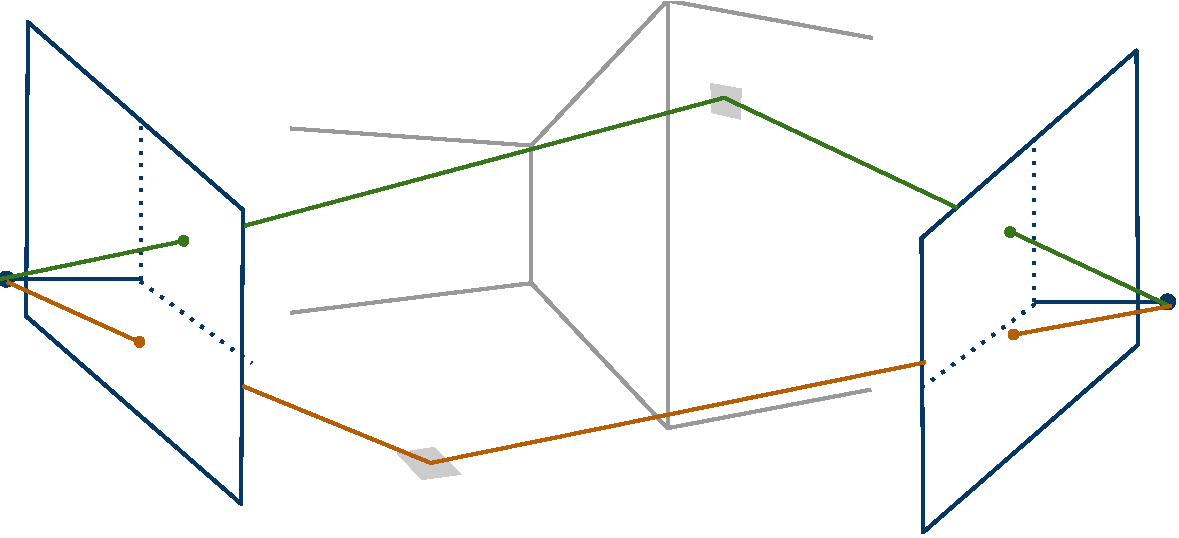
\includegraphics[width=0.4\textwidth]{figures/backproject}
  \caption{Pixel correspondences across multiple views are computed by
    back--projection into the world followed by re--projection in
    auxiliary views.}
  \label{fig:backproject}
\end{figure}

Need to show how to get $z$ coords of the planes.

\subsubsection{Extension: using orientation information}
Find floor and ceiling by maximizing NCC (weighted at bottom of
image?) w.r.t. floor and ceiling positions?

\subsubsection{Extension: using orientation information}

\subsubsection{EM for Occlusion Resolution}

\subsection{Depth features}


\begin{figure}[tb]
  \centering
  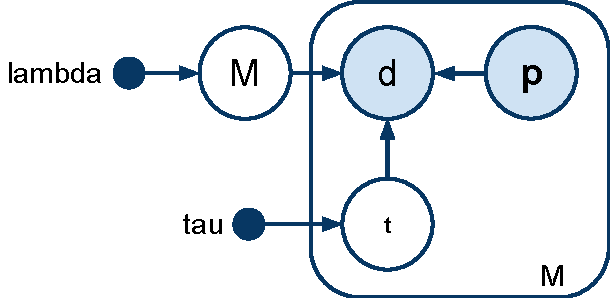
\includegraphics[width=0.5\textwidth]{figures/3d-gm}
  \caption{The graphical model relating indoor Manhattan models to 3D
    points. The hidden variable $t$ indicates whether the point is
    inside, outside, or coincident with the model.}
  \label{fig:monocular-gm}
\end{figure}

In this section we explore the context in which a 3D point cloud, as
generated perhaps by structure--from--motion or depth--sensing
hardware, is available to the system. For notational convenience we
assume that points are represented as pixel/depth pairs
$X=\{\Pixel_i,\Depth_i\}_{i=0}^N$. This representation is trivially
computed from a point cloud. We assume the following generative
model. First, an image point $\Pixel_i$ is sampled at random, then a
depth measurement $d_i$ is performed along the corresponding ray. The
relationship between $d_i$ and the model $M$ is determined by a hidden
variable $t_i\in\{\textsf{IN},\textsf{OUT},\textsf{ON}\}$ as follows:
\begin{enumerate}
  \item{If $t_i=\textsf{IN}$ then $\Depth_i$ corresponds to an object
    or surface within the room.}
  \item{If $t_i=\textsf{OUT}$ then $\Depth_i$ corresponds to an object
    or surface outside the boundary of the room, perhaps observed
    through a window or doorway. This case can also account for
    outliers generated at an earlier stage of processing.}
  \item{If $t_i=\textsf{ON}$ then $\Depth_i$ corresponds to the
    closest surface in $M$ in the direction of $\Pixel_i$.}
\end{enumerate}
We assign a fixed prior to $t$,
\begin{eqnarray}
  P(t=\textsf{IN}) = \tIN \hspace{0.5cm} 
  P(t=\textsf{OUT}) = \tOUT \hspace{0.5cm} 
  P(t=\textsf{ON}) = \tON ~.
\end{eqnarray}
We assume that each measurement is constrained to a known interval
$\left[0,d_{\textsf{max}}\right]$. Let $d_\Model(\Pixel)$ be the
depth to the nearest surface of model $M$ in the direction of
$\Pixel$ (see fig XXX). We model depth measurements accordinging to
\begin{eqnarray}
  \label{eq:x-inside}
  P(d~|~\Model,\Pixel,t=\textsf{IN}) &=&
  \begin{cases}
    \frac{1}{d_\Model(\Pixel)}, & \mbox{if } d_i < d_\Model(\Pixel) \\
    0, & \mbox{otherwise} \\
  \end{cases}\\
  \label{eq:x-outside}
  P(d~|~\Model,\Pixel,t=\textsf{OUT}) &=&
  \begin{cases}
    \frac{1}{d_{max}-d_\Model(\Pixel)}, & \mbox{if } d_i > d_\Model(\Pixel) \\
    0, & \mbox{otherwise} \\
  \end{cases}\\
  P(d ~|~ \Model,\Pixel,t=\textsf{ON}) &=&
  \mathcal{N}(d~;~d_\Model(\Pixel),\sigma)
\end{eqnarray}

\begin{figure}[tb]
  \centering 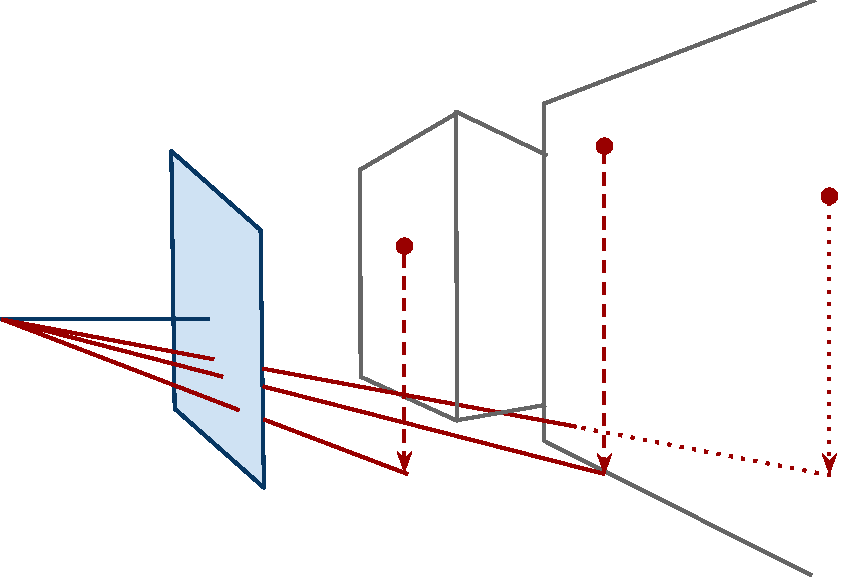
\includegraphics[width=0.4\textwidth]{figures/point-projs}
  \caption{Three possibilities for depth measurements: inside, outside, and
    coincident.}
  \label{fig:backproject}
\end{figure}

The posterior on $M$ is
\begin{eqnarray}
  \label{eq:3d-posterior}
  P(\Model~|~\Depths,\Pixels) &=& P(\Model) \prod_i P(\Depth_i,\Pixel_i~|~\Model) \\
  P(\Depth_i,\Pixel_i~|~\Model) &=& \sum_{t_i} P(\Depth_i,\Pixel_i,t_i~|~\Model) \\
  &=& \sum_{t_i} P(\Depth_i,~|~\Pixel_i,t_i,\Model) P(t_i~|~\Model) ~,
\end{eqnarray}
where in the second line we have omitted the prior on $\Pixel_i$ as it
is uniform over the image and will play no part in the maximisation to
come. Now \eqnref{3d-full-post} is a sum over three possible values
for $t_i$ and we can simplify this expression by distinguishing the
case where $d_i>d_\Model(\Pixel)$, in which case \eqnref{x-inside}
is $0$, from the case where the opposite is true, in which case
\eqnref{x-outside} is $0$. Hence,
\begin{eqnarray}
  \label{eq:3d-likelihood}
  P(\Depth_i~|~\Pixel_i,\Model) &=& \alpha +
  \tON \mathcal{N}(d_o~;~d_\Model(\Pixel),\sigma) \\
  \alpha &=&
  \begin{cases}
    \frac{\tIN}{d_\Model(\Pixel)}, & \mbox{if } d_i < d_\Model(\Pixel_i) \\
    \frac{\tOUT}{d_{max}-d_\Model(\Pixel)}, & \mbox{otherwise} \\
  \end{cases}~.
\end{eqnarray}

Notice that if the floor/wall intersection of a model $M$ meets column
$x$ at $y=y_f$, then this alone is sufficient to compute the depth
$d_(y';x,y_f)$ of the model at each pixel $(x,y')$ in that column. We
use this to express the posterior \eqnref{3d-posterior} in the payoff
form required by \eqnref{abstract-payoff}. Let $\mathcal{C}_x$ contain
indices for all depth measurements in column $x$, then
\begin{eqnarray}
  P(\Model ~|~ \Depths,\Pixels) &=& 
  \prod_{x} \prod_{i\in\mathcal{C}_x} P(\Depth_i~|~\Pixel_i,\Model) \\
  \log P(\Model ~|~ \Depths,\Pixels) &=& 
  P(M) + \sum_{x} \Bigl( \sum_{i\in\mathcal{C}_x}
  \log P(\Depth_i~|~\Pixel_i,y_f(x)) \Bigr) ~,
\end{eqnarray}
which we write in payoff form as
\begin{equation}
  \ColPayoff(x,y) = 
  \sum_{i\in\mathcal{C}_x} \log P(\Depth_i~|~\Pixel_i,y)
\end{equation}

TODO: explain where the prior on models went.

\subsection{Joint distribution}

We can trivially combine photometric, stereo, and depth data into a
joint model by assuming conditional independence between the sensor
modalities given $M$,
\begin{equation}
  P(M ~|~ X_{\textsf{mono}}, X_{\textsf{stereo}}, X_{\textsf{3D}})
  =  P(M) P(X_{\textsf{mono}} ~|~ M)
          P(X_{\textsf{stereo}} ~|~ M)
          P(X_{\textsf{3D}} ~|~ M) ~.
\end{equation}
Taking logarithms leads to simply summing over payoffs,
\begin{equation}
  \ColPayoff_{\textsf{joint}}(\vect{x}) =
  \ColPayoff_{\textsf{mono}}(\vect{x}) + 
  \ColPayoff_{\textsf{stereo}}(\vect{x}) +
  \ColPayoff_{\textsf{3D}}(\vect{x}) ~.
\end{equation}

\section{Inference}

\newcommand\OptModel{\Model^*}
\newcommand\PartialModel{\Model}
\newcommand\CroppedModel{\Model'}
\newcommand\PartialCol{x}
\newcommand\CroppedCol{x'}

We have reduced MAP inference to optimization over a payoff matrix:
\begin{equation}
  \OptModel = \argmax_\Model\limits \sum_x \ColPayoff\Bigl(x,y_f(\Model)\Bigr)
\end{equation}
Flint \etal \cite{FlintECCV10} showed that if an indoor Manhattan
model $\PartialModel$ is optimal over image columns
$\left[0,\PartialCol\right]$, then the ``cropped'' model
$\CroppedModel$, obtained by restricting $\PartialModel$ to the
sub--interval $\left[1,\CroppedCol\right]$, $\CroppedCol<\PartialCol$,
must be optimal over $\left[1,\CroppedCol\right]$. This permits a
dynamic programming solution in which the MAP model $\OptModel$ is
obtained by building up models from left to right.

Our algorithm differs from that of \cite{FlintECCV10} in that we do
not include the number of corners in the model as a state variable,
but instead accumulate the penalties $\Penalties$ each time we
consider adding a corner. This reduces complexity by $O(K)$, where $K$
is the number of walls in the model. We also operate directly on the
payoff matrix $\ColPayoff$, rather than by summing over pixel
agreements as in previous work. This is the key insight that allows 3D
and stereo data to be incorporated into the optimisation. For
completeness, we give the new recurrence relations below, though for
the full treatment the reader is referred to \cite{FlintECCV10}.
\begin{eqnarray}
  \label{eq:fout-recurrence}
    \fOUT(x,y,a) &=& \min_{a'\in\{l,r\}} \min
      \begin{cases}
        \fUP(x,y-1,a') + \PenaltyConc & \\
        \fDOWN(x,y+1,a') + \PenaltyOccl & \\
        \fIN(x,y,a') + \PenaltyOccl &
      \end{cases}\\
  \label{eq:fup-recurrence}
  \fUP(x,y,a) &=& \min \Bigl(\fIN(\cdot), \fUP(x,y-1,a)\Bigr)~,\\
  \label{eq:fdown-recurrence}
  \fDOWN(x,y,a) &=& \min \Bigl(\fIN(\cdot), \fDOWN(x,y+1,a)\Bigr)~,\\
  \label{eq:fin-recurrence-basic}
  \fIN(x,y,a) &=&
    \min_{x'<x}\Bigl(\fOUT(x',y',a)+ \Delta\Bigr) ~,\\
  \Delta &=& - \sum_{i=x'}^{x} \ColPayoff(i,y')\\
  \fOUT(0,y,a) &=& 0 \hspace{1cm} \forall y,a \\
  \fUP(x,0,a) &=& \infty \hspace{1cm} \forall x,a \\
  \fDOWN(x,N_x,a) &=& \infty \hspace{1cm} \forall x,a
\end{eqnarray}
XXX: These are useless, maybe just omit the recurrence relations? Or
move to appendix?

\section{Training}

Parameters to train from data
\begin{enumerate}
  \item{the penalties $\vect{\lambda}$ for the prior $P(M)$}
  \item{for monocular: the linear classifiers $\theta$}
  \item{for stereo: the photoconsistency metric $\Sigma$}
  \item{for 3D: the parameters $\vect{\tau}$ and the Gaussian
    variance $\sigma$.}
\end{enumerate}

\section{Results}


\bibliographystyle{splncs}
\bibliography{AVLstrings,VisionRefs}

\end{document}
